\clearpage
\section[Herleitung des Modells]{Ableitung des multimodalen Modells aus den gewonnen Interaktionszeiten}\label{sec:Herleitung}
Aus unserer Studie haben wir Zeiten für verschiedene Aktionen in den jeweiligen Kombinationen der Modalitäten erhoben.
Die Zeiten in den folgenden Tabellen sind Durchschnittszeiten für eine Aktion, der in einer bestimmten Kombinationen von Modalitäten ausgeführt wurde.
Wird eine Aktion in der Modalität Touch (T) ausgeführt gibt es drei mögliche Modalitäten, die nach einem Wechsel kommen können.
Entweder ebenfalls Touch und somit Touch\&Touch (TT) oder es folgt eine Moudswechsel zu Geste oder Sprache.
Die weiteren Kombinationen sind somit Touch\&Geste (TG) und Touch\&Sprache (TS).
Analog dazu haben wir Kombinationen bei denen Geste oder Sprache die erste Modalität ist.

Aus unseren Anwendungsbeispielen haben sich verschiedene Aktionen ergeben, die wir nun analysieren wollen, um daraus unser Modell abzuleiten.
In der folgenden Liste werden die einzelnen Aktionen der Anwendungsbeispiele erläutert (siehe auch Anwendungsbeispiele in \fref{fig:UseCases}):
\begin{itemize}
	\item \textbf{DA$_1$, DA$_2$:} Direktauswahl eines sichtbaren Elements auf dem ersten beziehungsweise zweiten Screen.
	Der erste Sreen beinhaltet vier Kacheln, die durch Symbole und Titel gekennzeichnet sind.
	Der zweite Screen beinhaltet drei Kacheln, die durch Text auf den Kacheln gekennzeichnet sind.
	\item \textbf{L$_1$, L$_2$ und L$_3$:} Der erste (zweite oder dritte) Swipe der Liste aus dem Anwendungsbeispiel Telefon.
	\item \textbf{DA (L):} Direktauswahl aus sichtbaren Elementen, nachdem im Anwendungsbeispiel Telefon bereits drei mal geswiped wurde und "`Maria Müller"' aus vier Elementen ausgewählt werden muss.
	\item \textbf{Inkr. (s)$_1$, Inkr. (s)$_2$ und Inkr. (s)$_3$:} Der erste (zweite oder dritte) Swipe der Wertinkrementation aus dem Anwendungsbeispiel Temperatur.
	\item \textbf{Inkr. (d)} Verschiebung des Sliders im Anwendungsbeispiel Medien.
	In der Modalität Sprache, entspricht dies dem Sprachbefehl "`achzig Prozent"'.
	\item \textbf{Popup:} Bestätigung des Popups, das nach dem Slider angezeigt wird.
	\item \textbf{1. Bu., 2. Bu., 3. Bu.:} Der Touch des ersten (zweiten oder dritten) Buchstaben im Anwendungsbeispiel Navigation.
	\item \textbf{Bu. >3:} Alle weiteren Buchstaben im Anwendungsbeispiel Navigation.
  \item \textbf{Maria M.:} Der Sprachbefehl "`Maria Müller"', der den Kontakt aus einer Liste direkt auswählt.
  Die Animationszeit, der scrollenden Liste wird nicht berücksichtigt (siehe R(Swipe)).
	\item \textbf{80 \%:} Der Sprachbefehl "`80\%"', um den Lautstärkeslider zu verstellen.
	\item \textbf{Wort S, M, L:} Kurzes Wort ("`Rom"'), mittellanges Wort ("`Dorfweg"') und langes Wort ("`Kirchengasse"').
	\item \textbf{OK:} Bestätigung der Zieleingabe im Anwendungsbeispiel Navigation.
	\item \textbf{R(Screen):} Konstante Zeit, die vom System benötigt wird von einem Screen auf den Nächsten zu wechseln.
	Ein Screenwechsel dauert 0,016 Sekunden.
	\item \textbf{R(Swipe):} Beim der Sprachmodalität wird nach dem Sprachbefehl: "`Maria Müller"' die Liste mit einer Animation zur richtigen Seite geswiped bevor der gewünschte Kontakt ausgewählt wird. Die Zeit dieser Animation nennen wir R(Swipe). Sie dauert in unserem Prototypen 1,5 Sekunden.
	\item \textbf{R(DA):} In der Modalität Sprache, wurde bei der DA nach jedem Sprachbefehl 0,5 Sekunden gewartet um die gelbe Markierung als Feedback zu geben. Diese 0,5 Sekunden müssen also bei DA$_1$ und DA$_2$ zur Gesamtzeit hinzugefügt werden.
\end{itemize}
Diese Einzelaktionen wollen wir in diesem Kapitel im Hinblick der Modalitätsunterschiede untersuchen und diese so weit es sinnvoll ist aggregieren, um ein übertragbares Modell zu bekommen.

Für die Sprachbefehle modellieren wir die Zeiten von verschiedenen Wortlängen.

Für uns am interessantesten in diesem Modell ist es, ob eine vorherige Modalität Einfluss auf die nachfolgende Modalität hat und ob und wie sich die Interaktionszeiten dadurch unterscheiden.
Die Zeiten wurden als Durchschnitt der Zeiten der 22 Probanden ermittelt.
Die Durchschnittszeiten aller Aktionen sind aus der \fref{tab:OperatorzeitenVorWechsel1}, \fref{tab:OperatorzeitenNachWechsel_TouchGeste} und \fref{tab:OperatorzeitenNachWechsel_Sprache} zu entnehmen.
\begin{table}[ht]
  \centering
	\begin{tabular}{|l|l|l|l|l|l|l|l|l|l|}
		\hline
		& \multicolumn{3}{|c|}{Touch (T)} & \multicolumn{3}{|c|}{Geste (G)}&\multicolumn{3}{|c|}{Sprache (S)}\\
		\hline
		Aktion 					& TT 		& TG 		& TS 		& GT 		& GG 		& GS 		& ST 		& SG 		& SS\\
		\hline
		DA$_1$ 	& 1,617 & 1,720	& 1,666 &	2,695	&	\textbf{2,595}	&	\textbf{2,833}	&	2,663	& 2,610	& 2,605\\
					&  			&  			&				&				&		\small{$(GS)^*$}					&	\small{$(GG)^*$}			 			&		&	& \\
		\hline
		DA$_2$ 	& 1,715 & \textbf{1,813}	& \textbf{1,728}	&	2,131	&	2,174	&	2,187	&	2,981	&	2,949	& 2,966\\
					&  			& \small{$(TS)^{**}$}				&	\small{$(TG)^{**}$}			&				&				&				&		&	& \\
		\hline
  \end{tabular}
	\caption[Durchschnittszeiten der Aktionen vor dem Wechsel einer Modalität]{Durchschnittszeiten in Sekunden der Aktionen vor dem Wechsel einer Modalität. Signifikanz wurde gemessen innerhalb einer Modalität vor dem Wechsel (zum Beispiel TT, TG und TS). Fettgedruckte Zeiten sind signifikant. Unter der Zahl steht zu welcher Kombination diese Zeit signifikant ist. Dabei gilt zusätzlich: * $\text{Signifikanz} \leq 0,05$, ** $\text{Signifikanz} \leq 0,01$ und *** $\text{Signifikanz} \leq 0,001$}
\label{tab:OperatorzeitenVorWechsel1}
\end{table}

\begin{table}[ht]
  \centering
	\begin{tabular}{|l|l|l|l|l|l|l|}
		\hline
		& 					\multicolumn{3}{|c|}{Touch (T)} & \multicolumn{3}{|c|}{Geste (G)}\\
		\hline
		Aktion 					& TT 	& GT 	& ST 	& TG 	& GG 	& SG 	\\
		\hline
		L$_1$				& $\textbf{1,518}$ 				& $\textbf{1,929}$				& $\textbf{1,893}$ 				&	1,902	&	$\textbf{1,797}$					&	$\textbf{2,190}$		\\
									& \small{$(GT, ST)^{***}$}	&	\small{$(TT)^{***}$}			& \small{$(TT)^{***}$}			&				&	\small{$(SG)^{**}$}				&	\small{$(GG)^{**}$}	\\
		\hline
		L$_2$			& 0,764 & 0,758	& 0,771 &	1,403	&	1,529	&	1,504 \\
		\hline
		L$_3$				& 0,884 & 0,883	& 0,818 &	1,271	&	1,336	&	1,191	\\
		\hline
		DA (L)				& 1,056 & 1,141	& 0,945 &	2,366	&	2,118	&	2,291	\\
		\hline
		Inkr. (s)$_1$				& $\textbf{1,453}$ 				& $\textbf{1,789}$		& $\textbf{1,726}$ 			&	1,672	&	$\textbf{1,536}$			&	$\textbf{1,745}$\\
									& \small{$(GT,ST)^{***}$} 	& \small{$(TT)^{***}$}	& \small{$(TT)^{***}$} 	&				&	\small{$(SG)^{***}$}		&	\small{$(GG)^{***}$}\\
		\hline
		Inkr. (s)$_2$				& 0,523 & 0,509	& 0,555 &	1,336	&	1,435	&	1,350\\
		\hline
		Inkr. (s)$_3$				& 0,552 & 0,583	& 0,561 &	1,279	&	1,266	&	1,361\\
		\hline
		Inkr. (d) 				& $\textbf{2,795}$ & $\textbf{3,365}$	& $\textbf{3,242}$ &	4,865	&	4,593	&	4,720\\
									& \small{$(GT,ST)^{**}$} & \small{$(TT){**}$}	& \small{$(TT){**}$}  &	&	&	\\
		\hline
		Popup 				& 0,778 & 0,795	& 0,777 &	$\textbf{1,335}$		&	$\textbf{1,067}$ &\\
									& 			& 			&  			&	\small{$(GG)^{*}$}	&	\small{$(TG)^{*}$} &		\\
		\hline
		1. Bu.  		& $\textbf{1,765}$ 						& $\textbf{1,990}$		& $\textbf{1,983}$ 	&				& 			&   \\
									& \small{$(GT)^{*},(ST)^{**}$}	& \small{$(TT)^{*}$}		& \small{$(TT)^{**}$}&			& 		& 	\\
		\hline
		2. Bu.  		& 0,613 & 0,647	& 0,664 &			& 			& 	 \\
		\hline
		3. Bu.  		& 0,631 & 0,633	& 0,662 &				& 			& \\
		\hline
		Bu. >3 			& \multicolumn{3}{|c|}{0,501}&				& 			& 	 \\
		\hline
		OK  					& 0,838 & 0,892 &	0,856 & 			& 			&  		\\
		\hline
  \end{tabular}
	\caption[Durchschnittszeiten der Aktionen nach dem Wechsel einer Modalität]{Durchschnittszeiten von Touch und Geste in Sekunden der Aktionen nach dem Wechsel einer Modalität. Signifikanz wurde gemessen innerhalb einer Modalität nach dem Wechsel (zum Beispiel TT, GT und ST). Fettgedruckte Zeiten sind signifikant. Unter der Zahl steht zu welcher Kombination diese Zeit signifikant ist. Dabei gilt zusätzlich: * Signifikanzniveau $\alpha \leq 0,05$, ** $\alpha \leq 0,01$ und *** $\alpha \leq 0,001$}
	\label{tab:OperatorzeitenNachWechsel_TouchGeste}
\end{table}

\begin{table}[ht]
  \centering
	\begin{tabular}{|l|l|l|l|}
		\hline
		& 					\multicolumn{3}{|c|}{Sprache (S)}\\
		\hline
		Aktion 					& TS 	& GS 	& SS\\
		\hline
		Maria M.
							&	$\textbf{2,961}$						& $\textbf{3,112}$							& $\textbf{2,802}$\\
							&	\small{$(GS)^{*},(SS)^{**}$}	& \small{$(TS)^{*},(SS)^{***}$}	& \small{$(TS)^{**},(GS)^{***}$}\\
		\hline
		80 \% 				&	$\textbf{3,126}$		& $\textbf{3,298}$ 							& $\textbf{2,914}$\\
									&	\small{$(SS)^{**}$}	& \small{$(SS)^{***}$} & \small{$(TS)^{**},(GS)^{***}$}\\
		\hline
		Popup 				&	1,941	& $\textbf{1,906}$ 		& $\textbf{2,100}$\\
									& 			& \small{$(SS)^{**}$} 	& \small{$(GS)^{**}$}\\
		\hline
		Wort S  			& $\textbf{2,627}$	& $\textbf{2,785}$		& $\textbf{2,346}$ \\
									& \small{$(SS)^{*}$}& \small{$(SS)^{***}$}	& \small{$(TS)^{*},(GS)^{***}$} \\
		\hline
		Wort M 				& 2,829 & $\textbf{2,956}$ 	& $\textbf{2,706}$ \\
									& 			& \small{$(SS)^{*}$} & \small{$(GS)^{*}$} \\
		\hline
		Wort L 				&	3,055	& 2,930	& 2,970\\
		\hline
		OK  					&	1,933	& 1,964	& 1,988\\
		\hline
  \end{tabular}
	\caption[Erste Vereinfachung der Durchschnittszeiten der Aktionen nach dem Wechsel einer Modalität]{Durchschnittszeiten von Sprachbefehlen in Sekunden der Aktionen nach dem Wechsel einer Modalität. Signifikanz wurde gemessen innerhalb einer Modalität nach dem Wechsel (zum Beispiel TT, GT und ST). Fettgedruckte Zeiten sind signifikant. Unter der Zahl steht zu welcher Kombination diese Zeit signifikant ist. Dabei gilt zusätzlich: * Signifikanzniveau $\alpha \leq 0,05$, ** $\alpha \leq 0,01$ und *** $\alpha \leq 0,001$}
	\label{tab:OperatorzeitenNachWechsel_Sprache}
\end{table}

Um das Modell zu verallgemeinern, fassen wir einige der Zeiten zusammen.
Alle Aktionen, die nicht unmittelbar nach einem Wechsel einer Modalität stattfinden, sollen zusammengefasst werden.
Die Aktionen unmittelbar nach einem Wechsel von Modalitäten sind L$_1$ (der erste Swipe aus den Kontakten), Inkr. (s)$_1$ (der erste Swipe, um die Temperatur zu inkrementieren), Inkr. (d) (Einstellung des Sliders) und 1. Bu. (der erste Touch des ersten Buchstaben).
All diese Aktionen weisen auch signifikante Unterschiede untereinander auf (siehe \fref{tab:OperatorzeitenNachWechsel_TouchGeste}, \fref{tab:OperatorzeitenNachWechsel_Sprache}).
Die Signifikanz wurde gemessen innerhalb einer Modalität nach einem potentiellen Wechsel.
Das heißt, die Interaktionszeiten der Modalität Sprache werden auf signifikante Unterschiede zur vorherigen Modalität untersucht (TS, GS und SS).
Fettgedruckte Zeiten sind signifikant.
Unter der Interaktionszeit steht, zu welcher Kombination diese Zeit signifikant ist.
Dabei gilt zusätzlich: * entspricht einem Signifikanzniveau von $\leq 0,05$, ** einem Signifikanzniveau von $\leq 0,01$ und *** einem Signifikanzniveau von $\leq 0,001$.

Als ersten fassen wir die Zeiten der direkten Auswahl (DA) zusammen, die vor einem Modalitätswechsel stattfinden und somit keinen Einfluss eines Wechsel haben können.
Für die Aktion DA$_1$ sehen wir signifikante Unterschiede zwischen der unimodalen Variante Geste (GG) und der multimodalen Variante Geste und Sprache (GS).
Im zweiten Screen gibt es ebenfalls einen signifikanten Unterschied in der Aktion DA$_2$ für Touch zwischen TS und TG (siehe \fref{tab:OperatorzeitenVorWechsel1}).
Wir werden die Interaktionszeiten trotzdem für jede Modalität zusammenfassen, da wir den möglichen Einfluss eines bevorstehenden Modalitätswechsels nicht berücksichtigen wollen.
Jetzt haben wir noch sechs verschiedene Durchschnittszeiten (jeweils Touch, Geste und Sprache für DA$_1$ und DA$_2$).

Die Zeiten von DA$_1$ und DA$_2$ unterscheiden sich.
Jedoch ist es schwer zu begründen welchen Variablen dieser Unterschied zugrunde liegt.
\begin{figure}[ht]
	\centering
		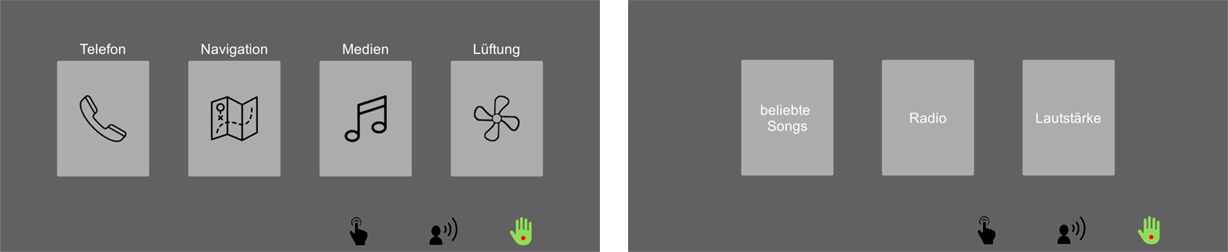
\includegraphics[width=1\textwidth]{img/Screen1vsScreen2.JPG}
	\caption{Unterschiedliche Varianten einer Direktauswahl}
	\label{fig:Screen1vsScreen2}
\end{figure}
Die Größe der Kacheln ist zwar gleich, jedoch ist die Anzahl der Kacheln unterschiedlich.
Es gibt auf dem zweiten Screen nur drei Kacheln, statt der vier Kacheln auf dem ersten Screen.
Außerdem sind im Hauptscreen Icons und Texte dargestellt, während auf dem zweiten Screen lediglich Texte abgebildet sind (siehe \fref{fig:Screen1vsScreen2}).
Wir wollen aber einheitliche Durchschnittszeit der drei Modalitäten für die Aktion Direktauswahl aus sichtbaren Elementen (DA), also die durchschnittliche Zeit, die für eine Auswahl von drei oder vier Kacheln der Größe 3,5cm x 4,5cm mit Text oder Icons benötigt wird.
Deshalb haben wir uns entschlossen die Zeiten zusammenzufassen (siehe \fref{tab:OperatorzeitenZusammengefasst1}).

Als nächstes fassen wir Aktionen zusammen, bei denen der Modalitätswechsel bereits stattgefunden hat.
Der erste Swipe findet beispielsweise unmittelbar nach einem potenziellen Modalitätswechsel statt.
Ein Modalitätswechsel beinhaltet meist einen Homing Operator wie im ursprüngliche Keystroke-Level-Modell.
Wechselt die Modalität zum Beispiel von Sprache zu Touch, muss die Hand vom Lenkrad genommen werden und sich zum Touchbereich bewegen.
Nach \citet{Green_2002} würde dies dem Operator $R_f$ (Reach Far) entsprechen.
Eine Aktion unmittelbar nach einem Modalitätswechsel dauert also länger, was sich durch die von uns ermittelten Zeiten auch bestätigen lässt.

Deshalb fassen wir für den zweiten und dritten Swipe der Liste (L$_2$), (L$_3$) die Modalität vor dem Modalitätswechsel zusammen.
Wir subtrahieren die Durchschnittszeit, die für einen zweiten oder dritten Swipe benötigt wird von (L$_1$) und bekommen damit die Vorbereitungszeit.
Diese Vorbereitungszeit enthält zum Beispiel eine Umpositionierung der Hand und eine mentale Vorbereitung auf die Aufgabe.
Es entsteht damit die einheitliche Aktion (L) für alle seitenweise Swipes und zusätzlich eine Vorbereitungszeit, die stets zum ersten Swipe addiert werden muss.
Die Vorbereitungszeit unterscheiden wir für jede Modalität und somit entsteht die Aktion V(L), siehe \ref{tab:OperatorzeitenNachWechsel3_TouchGeste}.
 
Dieses Vorgehen wenden wir analog für die Aktion Inkr. (s) an.
Auch hier ist der erste Swipe im Schnitt ca. eine Sekunde langsamer als die folgenden.
Wir wollen eine einheitliche Aktion Inkr. (s) und zusätzlich eine Vorbereitungszeit V(Inkr. (s)), die für die erste Ausführung benötigt wird.
 
Bei der Eingabe von Buchstaben per Touch unteilen wir die Zeiten zusätzlich in zwei Gruppen.
Wie wir bereits aus der Abbildung \ref{fig:Kategorien} abgeleitet haben gibt es auch hier eine deutlich längere Zeit für den ersten Buchstaben.
Zusätzlich nimmt die Zeit der Touch-Eingabe ab dem vierten Buchstaben nochmal deutlich ab (0,501 statt 0,642 Sekunden).
Wir modellieren zum einen eine Zeit für das Tippen der ersten drei Buchstaben und addieren für die Vorbereitung des ersten Buchstabens eine feste Zeit V(1. Bu) hinzu (analog zu den Aktionen L und Inkr. (s)).
Für alle weiteren Buchstaben verwenden wir eine weitere, geringere Durchschnittszeit (siehe \fref{tab:OperatorzeitenNachWechsel3_TouchGeste}).

Im nächsten Schritt werden wir unsere Aktionen für die Modalität Sprache noch vereinfachen, um unterschiedlich lange Wörter unterscheiden zu können.

Bei der Aktion Swipe Liste muss für die Modalität Sprache lediglich "`Maria Müller"' gesprochen werden, um in der Liste zur richtigen Position zu scrollen.
Bei der Aktion Inkr. (d) muss "`80 Prozent"' gesprochen werden, um den Slider auf 80 Prozent zu verschieben.
Da beides die Dauer darstellt, die benötigt wird um zwei Wörter auszusprechen, wollen wir diese Zeiten trotz signifikanter Unterschiede zusammenfassen (siehe \fref{tab:OperatorzeitenNachWechsel3_Sprache}).

Ähnlich dazu, wollen wir die Zeiten für Touch und Sprache des Bestätigungspopups und des "`Ok"'-Buttons verbinden und diese als einheitliche Aktion Bestätigung (B) zusammen fassen.
Sowohl bei Touch, als auch bei Sprache gibt es keine signifikanten Unterschiede zwischen dem Popup und dem "`Ok"'-Button.

Als letztes fassen wir die Wortlängen M ("`Dorfweg"') und L ("`Kirchengasse"') zusammen.
Diese sind beide signifikant unterschiedlich zur Wortlänge S ("`Rom"'), weisen aber untereinander keine signifikanten Unterschiede auf.
Die Unterscheidung der Modalitäten wird erhalten, da unmittelbar davor der Modalitätswechsel statt gefunden hat.
Bei diesen Aktionen wird somit lediglich unterschieden, ob sie einsilbig oder mehrsilbig sind.
Diese Aktionen kürzen wir daher ab mit Wort(e) für ein einsilbiges Wort und Wort(m) für ein mehrsilbiges Wort (siehe \fref{tab:OperatorzeitenNachWechsel3_Sprache}).

\begin{table}[ht]
  \centering
	\begin{tabular}{|l|l|l|l|l|l|l|l|l|l|}
		\hline
		& \multicolumn{3}{|c|}{Touch} & \multicolumn{3}{|c|}{Geste}&\multicolumn{3}{|c|}{Sprache}\\
		\hline
		Aktion 					& TT 		& TG 		& TS 		& GT 		& GG 		& GS 		& ST 		& SG 		& SS\\
		\hline
		DA 	& \multicolumn{3}{|c|}{1,710} &	\multicolumn{3}{|c|}{2,436} 	&	\multicolumn{3}{|c|}{2,795} \\
		\hline
  \end{tabular}
	\caption{Zusammengefasste Zeiten der Operatoren vor dem Modalitätswechsel}
\label{tab:OperatorzeitenZusammengefasst1}
\end{table}
\begin{table}[ht]
  \centering
	\begin{tabular}{|l|l|l|l|l|l|l|}
		\hline
		& \multicolumn{3}{|c|}{Touch (T)} & \multicolumn{3}{|c|}{Geste (G)}\\
		\hline
		Aktion 					& TT 	& GT 	& ST 	& TG 	& GG 	& SG \\
		\hline
		V(L)	& {0,705} 	& {1,116}		& {1,080} 	&	{0,530}		&	{0,425}		&	{0,818}\\
		\hline
		L					& \multicolumn{3}{|c|}{0,813} &	\multicolumn{3}{|c|}{1,372}\\
		\hline
		DA(L)			& \multicolumn{3}{|c|}{1,047} &	\multicolumn{3}{|c|}{2,258}\\
		\hline
		V(Inkr. (s))
										& {0,906} 	& {1,242}		& {1,179} 	&	{0,334}		&	{0,198}		&	{0,407}\\
										& \small{+ 0,547} 	& \small{+ 0,547}	& \tiny{+ 0,547} 	&	\small{+ 1,338}	&	\tiny{+ 1,338}	&	\small{+ 1,338}\\
		\hline
		Inkr. (s)				& \multicolumn{3}{|c|}{0,547} &	\multicolumn{3}{|c|}{1,338}\\
		\hline
		Inkr. (d)				& $\textbf{2,795}$ & $\textbf{3,365}$	& $\textbf{3,242}$ &	4,865	&	4,593	&	4,720	\\
									& \small{$(GT,ST)^{**}$} & \small{$(TT){**}$}	& \small{$(TT){**}$}  &	&	&		 \\
		\hline
		B 				& \multicolumn{3}{|c|}{0,829} &	\multicolumn{3}{|c|}{1,200}\\
		\hline
		V(1. Bu.)
										& {1,123} 	& {1,348}		& {1,341} 	&				& 			&  	\\
										& \small{+ 0,642} & \small{+ 0,642}	& \small{+ 0,642} &				& 			&  		\\
		\hline
		1-3. Bu.		& \multicolumn{3}{|c|}{0,642} &				& 			&  	 \\
		\hline
		Bu. >3 					& \multicolumn{3}{|c|}{0,501} &				& 		&  		\\
		\hline
  \end{tabular}
	\caption[Zweite Vereinfachung der Durchschnittszeiten von Touch und Geste nach dem Modalitätswechsel]{Durchschnittszeiten von Touch und Geste in Sekunden der Aktionen nach dem Modalitätswechsel. Signifikanz wurde gemessen innerhalb einer Modalität nach dem Wechsel (zum Beispiel TT, GT und ST). Fettgedruckte Zeiten sind signifikant. Unter der Zahl steht zu welcher Kombination diese Zeit signifikant ist. Dabei gilt zusätzlich: * Signifikanzniveau $\alpha \leq 0,05$, ** $\alpha \leq 0,01$ und *** $\alpha \leq 0,001$}
	\label{tab:OperatorzeitenNachWechsel3_TouchGeste}
\end{table}
\begin{table}[ht]
  \centering
	\begin{tabular}{|l|l|l|l|}
		\hline
		& \multicolumn{3}{|c|}{Sprache (S)}\\
		\hline
		Aktion 					&TS 	& GS 	& SS\\
		\hline
		2 Wörter		&	$\textbf{3,043}$						& $\textbf{3,205}$							& $\textbf{2,858}$\\
								&	\small{$(GS)^{*},(SS)^{**}$}	& \small{$(TS)^{*},(SS)^{***}$}	& \small{$(TS)^{**},(GS)^{***}$}\\
		\hline
		B						&\multicolumn{3}{|c|}{1,972}\\
		\hline
		Wort   		& $\textbf{2,627}$	& $\textbf{2,785}$		& $\textbf{2,346}$ \\
		(e)						& \small{$(SS)^{*}$}& \small{$(SS)^{***}$}	& \small{$(TS)^{*},(GS)^{***}$} \\
		\hline
		Wort  			& 2,917 & $\textbf{2,944}$ 	& $\textbf{2,839}$ \\
		(m)						& 			& \small{$(SS)^{*}$} & \small{$(GS)^{*}$} \\
		\hline
  \end{tabular}
	\caption[Zweite Vereinfachung der Durchschnittszeiten von Sprache nach dem Modalitätswechsel]{Durchschnittszeiten von Sprachbefehlen in Sekunden der Aktionen nach dem Modalitätswechsel. Signifikanz wurde gemessen innerhalb einer Modalität nach dem Wechsel (zum Beispiel TT, GT und ST). Fettgedruckte Zeiten sind signifikant. Unter der Zahl steht zu welcher Kombination diese Zeit signifikant ist. Dabei gilt zusätzlich: * Signifikanzniveau $\alpha \leq 0,05$, ** $\alpha \leq 0,01$ und *** $\alpha \leq 0,001$}
	\label{tab:OperatorzeitenNachWechsel3_Sprache}
\end{table}
\clearpage
\section[Multimodales Modell]{Multimodales Modell mit Wechselkosten}
In den vorherigen Schritten haben wir die gesammelten Durchschnittszeiten gruppiert und zusammengefasst.
Um die verschiedenen Aktionen mit ihren Interaktionszeiten übersichtlich zu einem Modell zusammenzufassen, betrachten wir ab jetzt die Aktionen vorerst unimodal (TT, GG und SS) und addieren je nach Modalitätswechsel die entsprechenden Wechselkosten hinzu.

Die unimodalen Interaktionszeiten waren stets schneller als die multimodalen Interaktionszeiten.
Wir verwenden diese als unsere Ausgangszeiten, indem wir sie von den Multimodalen Varianten subtrahieren.
Dadurch entstehen die sogenannten zusätzlichen Wechselkosten.
Zum Beispiel dauert die Aktion V(L) mit unimodaler Touch-Eingabe (TT) $0,705$ Sekunden und in der multimodale Variante Geste und anschließend Touch (GT) 1,116 Sekunden.
Ziehen wir die unimodale Zeit von der multimodalen ab, erhalten wir die Wechselkosten von $0,411$ Sekunden, die bei einem Wechsel von Geste zu Touch (W$_{GT}$) anfallen.

Wir haben die Aktion (DA) vor einem Modalitätswechsel für jede Modalität (ergibt 3 Aktionszeiten) und 13 Aktionen nach einem möglichen Modalitätswechsel für Touch und Geste (ergibt 17 Aktionszeiten) und 4 Aktionen nach einem möglichen Modalitätswechsel für Sprache identifiziert.
Dies ergibt 24 Aktionen und 20 verschiedene Arten von Wechselkosten.
Insgesamt kommen wir auf 44 verschiedene Interaktionszeiten für das multimodale Modell. Zusätzlich ergaben sich noch drei Antwortzeiten, die von unserem Prototypen anhängen.

In \fref{tab:DA} sind die zusammengefassten Zeiten der Aktion Direktauswahl aus sichtbaren Elementen, die vor dem Modalitätswechsel stattfinden. 
Die \fref{tab:AktionenUnimodal} listet alle Aktionen der drei Modalitäten mit ihren Interaktionszeiten auf.
Wird eine dieser Aktionen mit einer anderen Modalität ausgeführt als die vorhergegangene DA, müssen die Wechselkosten addiert werden.
Die dazugehörigen Wechselkosten für multimodale Interaktionen können aus \fref{tab:Wechselkosten} entnommen werden.

\begin{table}[ht]
  \centering
	\begin{tabular}{|l|l|l|l|l|l|l|l|l|l|}
		\hline
		& \multicolumn{3}{|c|}{Touch} & \multicolumn{3}{|c|}{Geste}&\multicolumn{3}{|c|}{Sprache}\\
		\hline
		Aktion 					& TT 		& TG 		& TS 		& GT 		& GG 		& GS 		& ST 		& SG 		& SS\\
		\hline
		DA 	& \multicolumn{3}{|c|}{1,710} &	\multicolumn{3}{|c|}{2,436} 	&	\multicolumn{3}{|c|}{2,795} \\
		\hline
  \end{tabular}
	\caption{Zusammengefasste Zeiten der Operatoren vor dem Modalitätswechsel}
\label{tab:DA}
\end{table}
\begin{table}[ht]
  \centering
			\begin{tabular}{|l|l|l|l|}
					\hline
				& \multicolumn{3}{|c|}{Unimodal}\\
				\hline
				Aktion 					& Touch & Geste & Sprache \\
				\hline
				V (L) 		& {0,705} 	&	{0,425}	&	\\
				\hline
				je (L)				& {0,813} &	{1,372} &\\
				\hline
				DA(L)						& {1,047} &	{2,258} & \\
				\hline
				V(Inkr. (s))		& {0,906} &	{0,198} &\\
				\hline
				Inkr. (s)			& {0,547} &	{1,338} &\\
				\hline
				Inkr. (d)					& {2,795} &	4,593 & \\
				\hline
				Bestätigung 		& {0,829} &{1,200} & {1,972}\\
				\hline
				V(1. Bu.)					& {1,123} 	& 	&\\
				\hline
				1-3. Bu.					& {0,642} & 	& \\
				\hline
				Bu. >3 					& {0,501}		&  	& \\
				\hline
				Wort(e)					& & & {2,346} \\
				\hline
				Wort(m) 				& & & {2,839}\\
				\hline
				2 Wörter 				& & & {2,858}\\
				\hline
			\end{tabular}
	\caption{Unimodale Interaktionszeiten.}
	\label{tab:AktionenUnimodal}
\end{table}

\begin{table}[ht]
  \centering
		\begin{tabular}{|l|l|l|l|l|l|l|}
				\hline
				& \multicolumn{6}{|c|}{Multimodalmodale Wechselkosten}\\
				\hline
				Aktion 					& Geste zu		& Sprache zu 	& Touch zu		& Sprache zu		& Touch zu		& Geste zu\\
												& Touch 			& Touch 			& Geste 			& Geste					& Sprache 		& Sprache \\
				\hline
				L$_1$ 					& ${+0,411}$ 	&	${+0,375}$	& ${+0,105}$ 	&	${+0,393}$		& \multicolumn{2}{|c|}{}	\\
				\hline
				Inkr. (s)$_1$		& ${+0,336}$ 	&	${+0,273}$ 	& ${+0,136}$ 	&	${+0,209}$		& \multicolumn{2}{|c|}{}	\\
				\hline
				Inkr. (d) 					& ${+0,570}$ 	&	${+0,447}$ 	& ${+0,272}$ 	&	${+0,127}$		& \multicolumn{2}{|c|}{}	\\
				\hline
				1. Buchstabe		& ${+0,225}$ 	& ${+0,218}$ 	&	\multicolumn{2}{|c|}{}			& \multicolumn{2}{|c|}{}	\\
				\hline
				Wort(e) 	& \multicolumn{2}{|c|}{}	& \multicolumn{2}{|c|}{}				& ${+0,281}$ 		& ${+0,439}$\\
				\hline
				Wort(m)	& \multicolumn{2}{|c|}{}	& \multicolumn{2}{|c|}{}				& ${+0,079}$ 		& ${+0,105}$\\
				\hline
				2 Wörter 				& \multicolumn{2}{|c|}{}	& \multicolumn{2}{|c|}{}				& ${+0,185}$ 		& ${+0,347}$\\
				\hline
			\end{tabular}
	\caption[Wechselkosten eines Modalitätswechsels]{Zusatzkosten (Wechselkosten) in Sekunden bei einem Modalitätswechsel. Diese Wechselkosten betreffen nur Aktionen direkt nach dem Modalitätswechsel. Wechselkosten müssen bei einem Modalitätswechsel dementsprechend aufaddiert werden.}
	\label{tab:Wechselkosten}
\end{table}

Zusätzlich zu den Interaktionszeiten ergeben sich noch drei Antwortzeiten:
\begin{itemize}
\item Die Zeit, die für das Laden des nächsten Screens benötigt wird mit einer Antwortdauer von 0,016 Sekunden.
\item Um dem Nutzer beim Anwendungsbeispiel Telefon Feedback zu geben, wurde für die Modalität Sprache, nach dem Sprachbefehl "`Maria Müller"' eine Animation eingebaut, die die Liste scrollen lässt, bevor der Kontakt markiert wird.
Diese Animation dauert 1,5 Sekunden.
\item Bei der Spracheingabe zur Direktauswahl aus sichtbaren Elementen wurde eine Verzögerung einer halben Sekunden eingebaut, um die Markierungsfarbe zu sehen.
\end{itemize}
Solche konstanten Antwortzeiten (Response Time) sind nicht übertragbar, und müssen für jedes zu testende Interface berechnet und in die Vorhersage miteinbezogen werden.
Für die Evaluation benötigen wir diese Zeiten.
\clearpage
\section[Qualitative Auswertung]{Qualitative Auswertung der Studie}
Eine qualitative Auswertung kann nicht in Zahlen ausgedrückt werden, sondern beinhaltet Kommentare der Probanden, sowie Beobachtungen des Studienleiters während der Studie.

Eine Studiendauer von 1,5 Stunden pro Proband stellte sich als sehr lange heraus.
Es konnte beobachtet werden, dass die Konzentration einiger Probanden mit der Zeit nach ließ.
Hinzu kam, dass es Anfang Dezember sehr kalt in der Parkgarage war.
Je nach Vorlieben konnte zwar die Sitzheizung eingeschaltet werden, jedoch wurden bei einigen Probanten mit der Zeit die Hände kalt.

Die Verwendung von Gesten als Eingabemodalität erwies sich als sehr unterschiedlich bei den Probanden.
Obwohl einige Schwierigkeiten bei der Gestenerkennung auftauchten, machte es den meisten sehr viel Spaß damit zu interagieren.
Es fiel auf, dass Probanden, bei denen die Gesteninteraktion sehr gut funktionierte, auch der Eindruck der Gesteninteraktionen deutlich positiver war.
Ein Grund weshalb die Gestenerkennung unterschiedlich gut funktioniert hat, war der festgelegt Interaktionsbereich zwischen Gangschaltung und Dashboard, siehe \fref{fig:GestenbereichSkizze}.
Die Einstellung des Sitzes und vor allem die Armlänge des Probanden, spielten eine Rolle, ob der Interaktionsbereich bequem erreicht werden konnte.
Probanden mit längeren Armen war es möglich diesen auf der Armlehne abzulegen und befanden sich dabei noch im Interaktionsbereich.
Unabhängig von der Armlänge zogen es manche Probanden vor, den Arm während der Gesteninteraktion frei in der Luft zu halten, was bei vielen eine gute Gestenerkennung ermöglichte.
Befindet sich die Hand jedoch zu weit hinten, kommen die Infrarotstrahlen des Leap Motion Controllers nicht durch die Gangschaltung und die Gestenerkennung funktioniert schlechter oder gar nicht.
Befindet sich der komplette Arm für eine Gesteninteraktion in der Luft, kann dieser bei längerer Dauer schwer werden, was das Ausführen der Gesten erschwert.

\begin{figure}[ht]
	\centering
		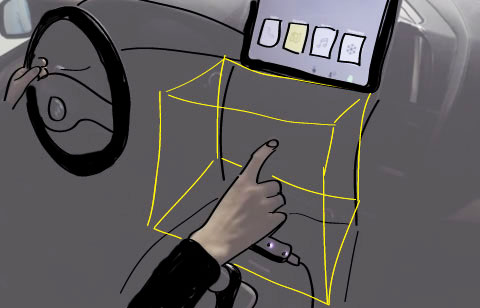
\includegraphics[width=1\textwidth]{img/GestenbereichSkizze2.jpg}
	\caption[Skizze des Interaktionsbereichs zur Gestenerkennung]{Grobe Skizze des Interaktionsbereichs zur Gestenerkennung. Die gelben Markierungslinien bilden den groben Bereich ab, in dem Gesten erkannt wurden.}
	\label{fig:GestenbereichSkizze}
\end{figure}

Bei der Touch-Eingabe ist aufgefallen, dass sie zwar keinerlei Schwierigkeiten bei der Interaktion verursachte, allerdings befand sich der Touchbereich etwas zu weit vom Fahrer entfernt.
Einige der Probanden mussten sich etwas nach vorne lehnen, um ihn optimal zu erreichen.
Dies stellt für die Bedienung im stehenden Auto kein Risiko dar, sollte jedoch während der Fahrt vermieden werden, um keine zusätzliche Ablenkung zu verursachen.

Aus den Kommentaren einiger Probanden lässt sich schließen, dass sie die Sprachbedienung für während der Fahrt am geeignetsten halten.
Andererseits wurde angemerkt, dass sie die Sprachbedienung eher allein im Auto nutzen würden als mit Mitfahrern.
Die multimodale Ausführung von Interaktionen kam insgesamt sehr gut an.
Immer wieder wurde jedoch angemerkt, dass haptische Bedienelemente für die Inkrementation besser geeignet wären.

\clearpage
\section[Diskussion]{Diskussion zur Studie und Erstellung des Modells}
Bei der Entwicklung des Prototypen und der Erhebung der Interaktionszeiten aus der Studie gab es einige Einschränkungen und Entscheidungen, die im Zusammenhang der Studienergebnisse im folgenden diskutiert und interpretiert werden.

Aus den Ergebnissen der Studie wurden die durchschnittlichen Interaktionszeiten für insgesamt 24 Aktionen und 20 verschiedene Arten von Wechselkosten abgeleitet. 
Die Interaktionszeiten für die Aktionen, die per Touch-Eingabe getätigt werden sind, verglichen mit Geste und Sprache, am schnellsten. 
Für die Vorbereitungszeiten (V(L)) und V(Inkr. (s)) für die Touch-Eingabe, benötigten die Probanden allerdings länger als bei der Vorbereitung für Gesten dieser Aktionen.
Das liegt an dem Interaktionsbereich, der für Gesteninteraktionen näher positioniert ist als der für die Touch-Eingabe. 
Das deckt sich mit Fitts`Law, dass für eine weitere Distanz, ein zu treffenden Zieles längere Zeiten benötigt. 

Als erste Einschränkung haben wir die Interaktion mit klassischen haptischen Bedienelementen aus unserer Studie ausgeschlossen.
Dies lag dem großen Mehraufwand zugrunde, der dabei entstanden wäre.
Um haptische Bedienelemente befriedigend zu modelliere, müssten, um nur ein Beispiel zu nennen, verschiedene Drehwinkel eines Drehrades gemessen werden \citep{schneegass_2009}.
Allein durch unsere drei Modalitäten mit Touch, Sprache und Geste entstand ein Studienumfang von 1,5 Stunden pro Teilnehmer, in der alle Kombinationen der drei Modalitäten getestet wurden.
Wir haben uns deshalb entschieden, uns in dieser Arbeit auf die Modalitäten Touch, Sprache und Geste zu fokussieren.

Die Bedienung im Auto durch haptische Knöpfe, Schalter und Regler ist und bleibt ein wichtiger Bestandteil, um Funktionen im Auto zu betätigen.
Ein großer Vorteil ist hierbei, dass die Eingabe nahezu blind getätigt werden kann, ohne die Aufmerksamkeit von der Straße zu lenken.
Die Verwendung von haptischen Bedienelementen im Auto wurde bereits in vorherigen Studien untersucht \citep{Pettitt_2007,schneegass_2009,SchneegaB_2011}.

In der Studie zur Erhebung von multimodalen Interaktionszeiten verwenden wir keine Fahraufgabe.
Stattdessen messen wir die Gesamtdauer (Total Task Time), die in einem stehenden Auto benötigt wird um eine Aufgabe zu lösen.
Um den Grad der visuellen Ablenkung, solcher multimodalen Interaktionen messen zu können, sollte unser Modell zusätzlich noch dahingehend erweitert werden, die visuelle Ablenkung miteinzubeziehen \citep{Pettitt_2007}.
 
Um für alle Kombinationen ausreichend Zeiten erheben zu können musste jeder Nutzer im within-subject Design alle 33 Kombinationen durchführen.
Da wir in unserem Modell, wie bei dem Keystroke-Level-Modell \citep{Card_1980}, von Experten ausgehen wollen, mussten die Probanden vorher die Interaktion üben.
\citet{Jude:2014} zeigte in seiner Arbeit zu multimodaler Interaktion von Geste und Sprache, dass eine sehr schnelle Interaktionssteigerung mit relativ geringem Training zu beobachten ist.
Außerdem entschlossen wir uns von jedem Probanden zwei Messdurchgänge zu erheben, um somit die Durchschnittszeit beider Messdurchgänge verwenden zu können.
Diese Vorkehrungen bedeuteten allerdings, dass die Studiendauer bis zu 1,5 Stunden pro Durchlauf betrug (abhängig von der Anzahl der Probedurchgänge).

Durch die Permutation aller Modalitäten und Anwendungsbeispielen sollten eventuelle beeinflusssende Effekte auf alle Varianten gleichermaßen verteilt werden.

Die Vorerfahrung von Sprache ergab im Durchschnitt einen Wert von 2,32, bei Touch 3,95 und bei Geste 1,86.
Die große Erfahrung mit der Touchbedienung lässt sich auf die weitverbreitete Smartphonenutzung zurückführen.
Mit der Gestensteuerung haben die Probanden wie erwartet die geringste Erfahrung.
Acht der 22 Probanden hatten keine Erfahrungen mit der Gestensteuerung und keiner davon nutzt sie regelmäßig.
Diese Erfahrungswerte liegen der wenig verbreiteten Anwendungen mit Gesteninteraktionen zu Grunde die der Endnutzer bisher lediglich in der XBox Kinect von Microsoft findet.

Für die Sprachmodalität haben wir nicht alle Aktionen abgebildet.
Statt zum Beispiel in einer Liste aus Kontakten durch einen Sprachbefehl "`nächste Seite"' zu scrollen , erschien es uns geeigneter direkt den Kontakt "`Maria Müller"' auszuwählen.
Ebenso wurde beim Einstellen der Temperatur oder der Lautstärke der gewünschte Wert direkt, das heißt ohne Inkrementation, gesprochen.

In unserem multimodalen Modell unterscheiden wir für die Modalität Sprache nur zwischen einsilbigen und mehrsilbigen Wörtern, sowie einer Durchschnittszeit von zwei Wörtern.
Die Aktion "`2 Wörter"' wurde aus dem Sprachbefehl "`Maria Müller"' und "`80 Prozent"' gebildet, obwohl signifikante Unterschiede vorlagen.
Diese Entscheidung wurde getroffen, um eine übertragbare Aktion für andere Prototypen zu erhalten.
In den meisten gängigen Informationssystemen im Auto, die Sprachbedienung verwenden, können ganze Sätze gesprochen werden (zum Beispiel "`navigiere in die Kirchengasse Nummer 17"').
Um die Vorhersage für Dauer eines Satzes zu modellieren müsste unser Modell noch dahingehend genauer untersucht und erweitert werden.

Die Zeit der Touch-Eingabe, ab dem vierten Buchstaben nimmt nochmal deutlich ab (0,501 statt 0,642 Sekunden), weshalb wir diese als eigene Aktionszeit definiert haben.
Zu diesem Zeitpunkt hat sich der Nutzer bereits mit der Tastatur vertraut gemacht und wodurch die weitere Eingabe schneller verläuft.
Das Inputfeld im Screen der Texteingabe befand sich unter der Tastatur und wurde bei einer Touch-Eingabe durch die Hand verdeckt.
Das Feld sollte sich besser über der Tastatur befinden.

Die Aktion Direktauswahl aus sichtbaren Elementen sollte so erweitert werden, dass sie auch nach einem Wechsel modelliert stattfinden kann.
In unseren Anwendungsbeispielen kam diese Variante nicht vor und konnte somit nicht modelliert werden.

Der Gesteninteraktionsbereich war nicht für alle Probanden optimal, je nach Armlänge konnten die Gesten der Probanden besser und schlechter ausgeführt werden.
Probanden, bei denen sich der Interaktionsbereich zu weit weg befand, mussten sich mehr darauf konzentrieren die Geste richtig auszuführen, was die Interaktion verlangsamte und die potenzielle Ablenkung erhöhte.
\citet{Riener:2013:SIG} untersucht in eine Studie den Bereich für Gesten.
Sie stellten fest, dass die häufigste Gesteninteraktion sich in dem Dreiecks-Bereich von Lenkrad, Rückspiegel und Gangschaltung befindet.
Unsere Gestenerkennung befand sich somit innerhalb dieses Bereichs.
Es wäre wünschenswert, dass dieser Interaktionsbereich Bereich individuell einstellbar ist, um die Gestenerkennung so bequem und robust wie möglich zu gestalten.

Auch das Touchdisplay war für einige Probanden zu weite entfernt positioniert.
Dieses sollte für den Fahrer ohne große Anstrengung erreichbar sein.
Zur Optimierung der Interaktion mit großen Touchdisplays haben \citet{Rumelin:2013} Touchvarianten verglichen und zum Beispiel ein haptisches Element als Orientierungshilfe in den Screen eingebaut.
Mit ihm kann die Interaktion eines Kuchenmenüs von diesem Punkt aus fast blind getätigt werden.
Um visuelle Überlagerungen von Karten zu verbessern haben \citet{lee2013saliency} die Suche von Elementen durch die präattentive Wahrnehmung durch das Hervorheben von Elementen verbessert und konnten somit Ablenkungen reduzieren.
Es gibt also nicht nur für die Kombination von Modalitäten, sondern auch für jede einzelne Modalität noch Verbesserungspotenzial.

Grundsätzlich lässt sich sagen, dass die Sprachbedienung am beliebtesten bei den Probanden war.
Jedoch wurde oft angemerkt, dass sie diese Modalität nicht mit Mitfahrern verwenden würden.
Dies unterstreicht unsere Annahme, dass es sinnvoll ist bei einem IVIS mehrere Modalitäten anzubieten.
Nach der reinen Sprachbedienung war die zweitbeliebteste Kombination Touch und Sprache, dicht gefolgt von Geste und Sprache.
Das zeigt, dass multimodale Interaktionen durchaus gewünscht sind, was auch von den Kommentaren bestätigt wurde.

Die Aktionen unseres multimodalen Modells sind nicht so feingranular wie die Operatoren aus dem Keystroke-Level-Modell, sondern befinden sich eine Ebene höher.
Statt separate Zeiten für die mentale Vorbereitung, der Bewegung vom Lenkrad zum Interaktionsbereich und der Bewegung innerhalb eines Interaktionsbereichs zu modellieren, haben wir diese als durchschnittliche Vorbereitungszeit für drei verschiedenen Aktionen je nach Modalität zusammengefasst.
Für der Modellierung des Keystroke-Level-Modell wird genau vorgegeben, wann der Experte welche Bewegung macht und wann er sich mental vorbereitet.

Diese Herangehensweise hielten wir für unser Modell für zu genau und hätte außerdem per Videoanalyse ausgewertet werden müssen.
Um die Akkudauer der GoPro-Kamera zu verlängern, haben wir die Auflösung verringert.
Die Bildqualität reichte aus, um die Varianten nachzuvollziehen, für eine Videoanalyse zur Bestimmung von Operatoren ist sie allerdings ungeeignet.
Es wurden über 22 Stunden Videomaterial aufgenommen.

Unser multimodales Modell enthält Aktionszeiten, die ein geübter Nutzer im Durchschnitt benötigt, um eine bestimmte Aktion in einer bestimmten Modalität auszuführen.
Das Modell soll eine grobe Abschätzung der Interaktionszeiten in Abhängigkeit der Modalität mit Berücksichtigung der Wechselkosten berechnen.
Diese Vorhersage einer multimodalen Interaktionsdauer soll Vergleiche zwischen verschiedenen Kombinationen von Modalitäten der Aktionen ermöglichen.
Es ist jedoch zu erwarten, dass die Vorhersagen der Interaktionszeiten eventuell nicht so präzise sind, wie die eines Keystroke-Level-Modells.